After the first MapReduce phase is completed, the skyline candidate object set $O_c$ is collected. In the next step, the final skyline probability is needed to be computed for determining $p-$skyline object set. In the first MapReduce phase, the angle-based processing only knows the local data at a fixed angle region, and objects remained after pruning decide the final step of merging. Before illustrating our merging algorithm for computing skyline probability, we study the distribution shape of remained candidate objects after the first MapReduce phase.
\subsection{Shape Analysis}

\begin{figure*}[!t]
    \begin{center}
    \vspace{-1.5pc}
  \subfigbottomskip = 2pt \subfigure[Independent Distribution]
    {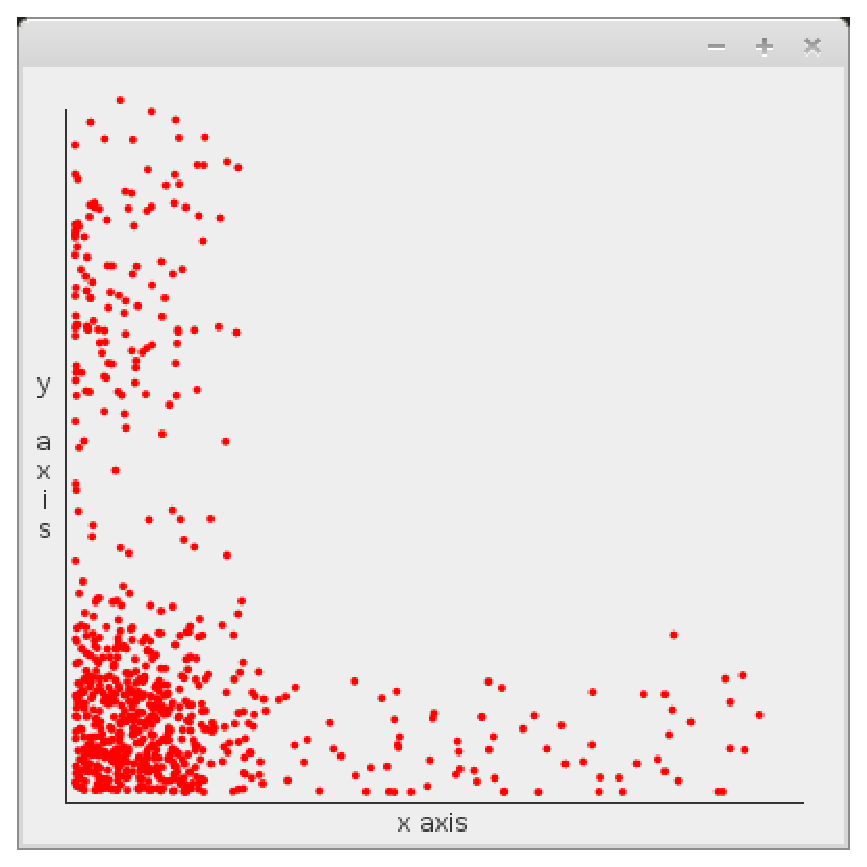
\includegraphics[width=0.24\textwidth]{figs/inde.eps}}
    \hspace{0.01em}
  \subfigbottomskip = 2pt  \subfigure[Anti-correlated Distribution]
    {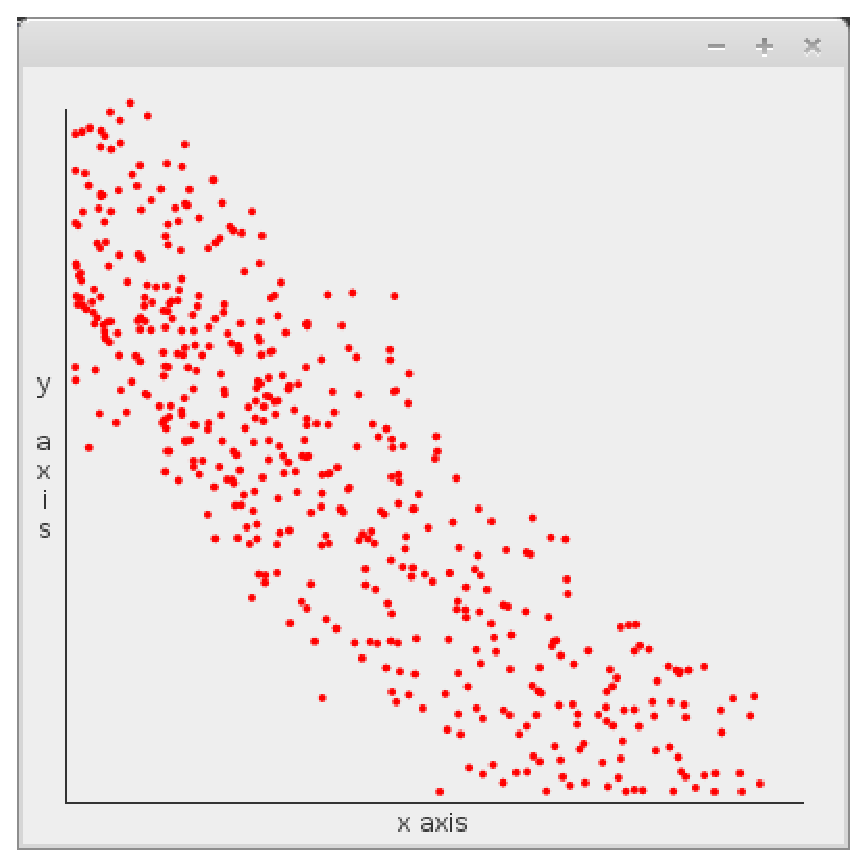
\includegraphics[width=0.24\textwidth]{figs/anti.eps}}
    \hspace{0.01em}
  \subfigbottomskip = 2pt  \subfigure[Correlated Distribution]
    {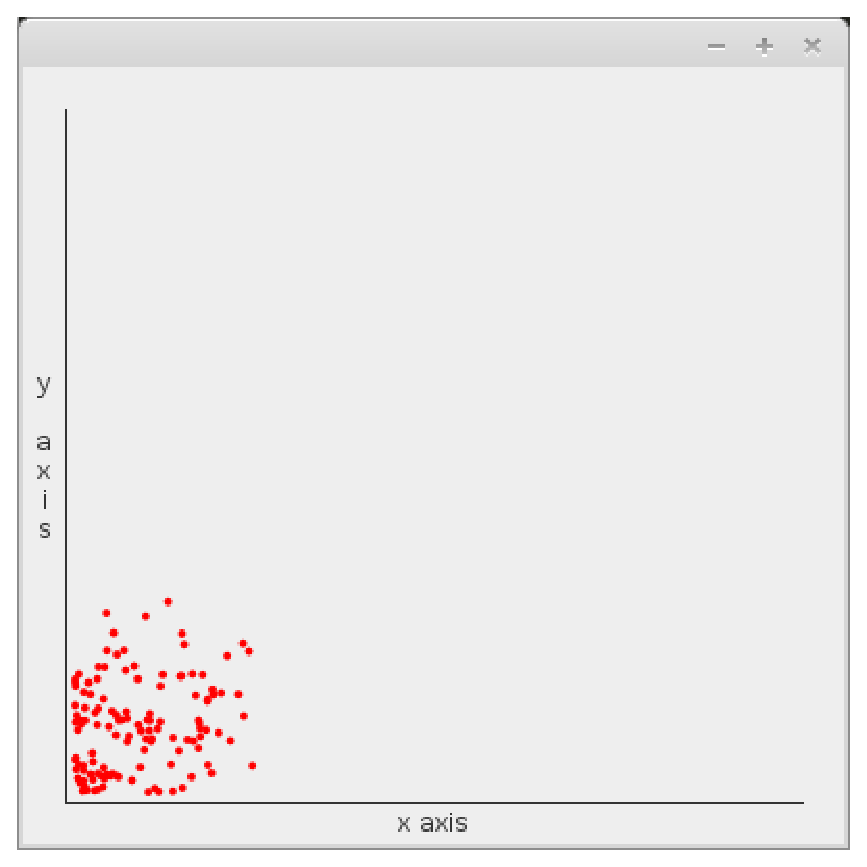
\includegraphics[width=0.24\textwidth]{figs/corr.eps}}

    \caption{Data Point Distribution after phase 1.}
    \label{fig:shape}
    \end{center}
\vspace{-10pt}
\end{figure*}

An experiment is conducted to depict the shape of instance distribution. The detailed experiment environment is illustrated as follows. In the two-dimensional space, objects are distributed between [0, 1] in domain of each dimension. Three varieties of object distribution (independent distribution, correlated distribution, and anti-correlated distribution) are tested respectively. The cardinality of objects is 5000. For each object, instances are created under a rectangle region, the edge size of which follows a normal distribution in range [0, 0.2] with expectation 0.1 and standard deviation 0.025.
The number of instances in each object follows uniform distribution in range [1, 100, and the first quadrant is evenly splitted into 6 angles. We apply the pruning algorithm in the first phase, filter objects which could not be in the $p$-skyline set. After that, we collected the objects which are still remained in each region, and paint all of them in the x-y axis. Figure~\ref{fig:shape} showed the result. For Independent or Anti-correlated data, many instances are remained. Therefore, the Strategy proposed in the merging phase should be able to apply for any variety of data distribution, especially for Independent and Anti-correlated data.

\subsection{Rectangle Splitting}
\begin{figure}[t]
\vspace{-15pt}
\centering
  \centerline{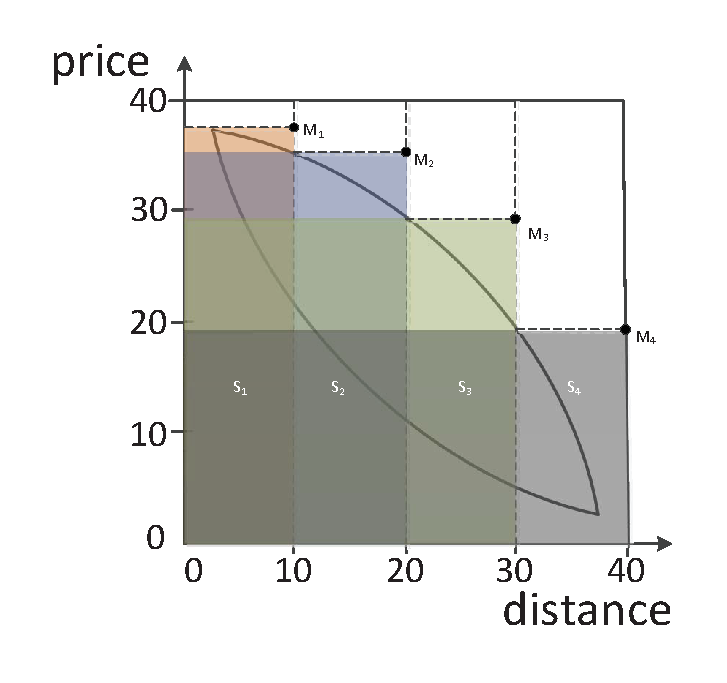
\psfig{file=figs/grid-merge.eps,width=3.0in}}
  \caption{Merging Phase}
  \vspace{-15pt}
  \label{figure:gridMerge}
\end{figure}

In this section, we propose an approach to efficiently evaluate skyline probability for  remained candidate objects. To utilize the MapReduce framework, we partition remained data to several domains which are able to work individually. The intuitive idea is to split data into several partitions, and each partition is not affected by others. Take Figure~\ref{figure:gridMerge} as an example. Data is distributed like spindle shape. Rectangles of different colors are drawn and any instance is covered by at least one rectangle. Data covered by a rectangle is sent to separate machine. It is found that object candidates in a machine are only dominated by instances in this rectangle. Then skyline probability is easily computed only regarding this partition. In Figure~\ref{figure:gridMerge}), the whole space is split into 4 parts $S_1, S_2, \dots, S_4$ based on X axis evenly partitioned. The maximum corner points (maximum coordinate in every dimension) is collected for each partition. Each maximum corner point denoted by $M_i$, is dominated by any instance in $S_i$. Then each grid region is rounded by the origin and the maximum point. In Figure~\ref{figure:gridMerge}, $S_3$ (green area) represents instances in a rectangle from the origin to $M_3$.

%
% using dynamic mapping strategy to let I_1 *C_o_1 = I_2 * C_o_2
%
The map phase is to send necessary data to reducers.
Recall that we have two remained sets of data, object set $C_o$ and instance set $I_p$. To avoid repeatedly computing, we propose a dynamic mapping strategy to send data to separate reducer evenly. Followed by the example, data is partitioned along the x-axis. Given the the number of reducers $n$, the data is partitioned into n parts.
Every partition has two types of data, instances in $C_o$ and $I$ respectively, representing object candidates and influenced instances respectively. Take Figure~\ref{figure:gridMerge} as an example. The instances of $C_o$ in $S_2$ is in $S_2$ rectangle, and instances in the blue area are instance set $I$, which dominates $C_o$. Based on the grouping scheme, the mapping phase maps the two types of data to every slave machine. It is obvious that the choice of $n$ affects the efficiency of skyline probability computing. In the experiment section, the performance trend with the variety of $n$ is observed.

In the reduce phase, skyline probability of every instance is computed. Assume an instance $p$ is in a partition $V^A$. Since $p$ is only dominated by corresponding region of instances, the instance skyline probability $SkyProb(p)$ is obtained using the standard approach.  It iterates all instances in this partition, and do skyline probability computation introduced in the Section~\ref{sec:prelim}. Then instance skyline probability of all instances is outputed for each partition. 

After every instance in $C_o$ obtains its instance skyline probability, the second phase is completed. object skyline probability is grouped by iterating all instance skyline probability by Equation~\ref{equ_final}. $p-$skyline object set is easily obtained by retrieving objects whose object skyline probability is larger than or equal to $p$.

